
\documentclass{article}

\usepackage[margin=1in]{geometry} 
\usepackage[french]{babel}
\usepackage[T1]{fontenc}
\usepackage[utf8]{inputenc}
\usepackage{amsmath,amsthm,amssymb,amsfonts, fancyhdr, color, comment, graphicx, environ}
\usepackage{xcolor}
\usepackage{mdframed}
\usepackage[shortlabels]{enumitem}
\usepackage{indentfirst}
\usepackage{hyperref}
\usepackage{lastpage}
\usepackage{listingsutf8}
%\usepackage{ff++listings}
\usepackage{amsmath}
\DeclareMathOperator{\Tr}{Tr}

\usepackage{physics}
\usepackage{amsfonts}
\usepackage{float}
\PassOptionsToPackage{hyphens}{url}\usepackage{hyperref}

\usepackage{xurl}

\renewcommand{\footrulewidth}{0.8pt}
\hypersetup{
    colorlinks=true,
    linkcolor=blue,
    filecolor=magenta,      
    urlcolor=blue,
}

\pagestyle{fancy}

\newenvironment{problem}[2][Etape]
    { \begin{mdframed}[backgroundcolor=gray!20] \textbf{#1 #2} \\}
    {  \end{mdframed}}

\newenvironment{solution}{\textbf{Réponse}}

\lhead{L. Gomes et F. Pollet}
\rhead{ES Elements finis} 
\chead{\textbf{Optimisation de l'épaisseur d'un pont}}
\lfoot{D. Ryckelynck, N. Spillane, P.-H. Tournier}
\cfoot{Mines Paris}
\rfoot{\thepage/\pageref*{LastPage}}


\begin{document}

    \title{\Large ES Elements Finis  \\[0.5cm]
        \bf\Large Optimisation de l'épaisseur d'une structure tridimensionnelle}
\author{\large Leticia Gomes\\Pollet Florent \ \\}
\date{\large\today}

\makeatletter
    \begin{titlepage}
        \begin{center}
	   { 
\includegraphics[width=12cm]{mp_logo.png}}
	   {\ \\ \ \\}
        \vbox{}\vspace{5cm}
            {\@title }\\[3cm] 
            {\@author}
            {\large \ \\ Encadrants: \bf David Ryckelynck, Nicole Spillane et Pierre-Henri Tournier\\ \ \\}
            {\@date\\}

        \end{center}
    \end{titlepage}

    \tableofcontents

    \clearpage
\makeatother%not necessary but looks fancy

    % rappel du problème ? reprendre photo du sujet
    % référence à la fin
    % appendix pour code ?

    \section{Présentation du problème}
    La méthode des éléments finis est une méthode matématique utilisée par industriels et chercheurs afin de résudre numériquement des équations aux dérivées partielles. Une application envisageable pour les calculs avec la méthode des éléments finis est l'optimisation de l'épaisseur d'une structure tridimensionelle, 
    qui est ainsi l'objectif de ce projet. 
    La structure tridimensionnelle choisie est un pont pour lequel nous avons cherché à minimiser l'épaisseur
    en respectant une contrainte de déplacement vertical maximal en son centre de $10$ cm malgré l'application d'une force surfacique
    constante sur la surface horizontale supérieure du pont. 
    La géométrie de ce problème est tridimensionnelle et sa coupe verticale est montré dans la Figure \ref{fig:problem}.
    \begin{figure}[H]        
    \begin{center}
	
        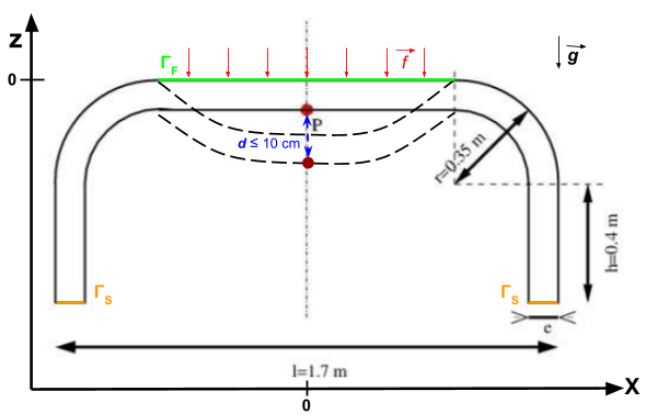
\includegraphics[width=12cm]{imgs/coupe_2D-schema.JPG}
        \caption{Schéma de la géométrie du pont. Une force surfacique $f= - 5x10^8 N m^(-2)$ est appliquée à sa surface supérieure. Le déplacement maximale $d$ est montré en bleue, en vert c'est $\gamma$F, surface dans lequelle la force est appliquée et $\gamma$S est la surface inférieure fixe. Le système est qui est soumis à la gravité $g$.}
        \label{fig:problem}
    
	\end{center}
    \end{figure}
    
    La structure est considérée comme homogène avec les extrémités inférieures fixes et une largeur $p = 0,5 m$. 
    
    Les données fournis pour ce système sont :
    
    \begin{itemize}
    \item Module d'Young : $E = 2.1 \times 10^11$ N m$^{-2}$
    \item Coefficient de Poisson : $\nu = 0.3$ 
    \item Masse Volumique : $\rho = 7800$ kg m$^{-3}$
    \item Force imposée sur le bord supérieur : $f= - 5 \times 10^8$ N m$^{-2}$
    \end{itemize}
    
    Nous avons adopté la stratégie suivante pour traiter ce projet, en trois parties :
    \begin{enumerate}
        \item Établissement de la formulation variationelle pour ce problème ;
        \item Résolution à épaisseur fixée : nous avons écrit un programme avec la langage FreeFem++ pour résoudre le système à épaisseur fixe $e = 0,1 m$, 
            avec une maille initialement bidimentionelle qui est ensuite complétée avec la fonction $buildlayers$. 
            Nous avons étudié la différence entre des solutions calculées pour la pièce et pour sa moitié ainsi que la précision du résultat en variant le maillage.
        \item Optimisation de l'épaisseur :
        \begin{enumerate}
            \item Approximation graphique : 
                nous avons analysé la relation entre l'épaisseur et le déplacement afin de trouver un intervalle où le déplacement est inférieur ou égal à 10 cm.
            \item Raffinement de la solution : nous avons utilisé la méthode de dichotomie pour résoudre le système.
        \end{enumerate}
    \end{enumerate}

    \newpage
    
    \section{Formulation variationnelle}

    \begin{problem}{1}
    Mettons le problème sous forme faible (variationnelle) pour pouvoir le résoudre avec la méthode des éléments finis.
    \end{problem}
    
    \begin{solution}   
        On part de la formulation forte. On cherche le déplacement $\vec{u}$, fonction de $\mathbb{R}^3$ dans $\mathbb{R}^3$.

Pour cela, on réalise d'abord un bilan des forces sur le système étudié qui est le pont dans le référentiel terrestre. Le système est à l'équilibre donc $\vec{a} = 0$.

On définit

\begin{equation}
    \vec{f} = \begin{pmatrix} 0\\ 0\\ f\\\end{pmatrix}
\end{equation}

et sa valeur est spécifiée dans l'énoncé.

On définit 

\begin{equation}
    \vec{g} = \begin{pmatrix} 0\\ 0\\ -g\\\end{pmatrix}
\end{equation}

où $g$ est l'accélération de la pesanteur standard.

On se place en 3D. On définit le domaine $\Omega$ comme l'ensemble du pont (qui est un polygone), et la frontière $\Gamma$ est partitionnée comme selon le schéma.

Le schéma n'est pas à l'échelle.

D'après le cours de mécanique,

\begin{equation}
    \begin{cases}
        \lambda = \frac{E}{2(1+\nu)}\\
        \mu = \frac{\nu E}{(1+\nu)(1-2\nu)}
    \end{cases}
\end{equation}

et on cherche donc $\vec{u} \in \mathcal{C}^2(\bar{\Omega})^3$ tel que

\begin{equation}\label{fort}
    \begin{cases}
      \div \sigma + \rho \vec{g} = 0 \textrm { sur $\Omega$ (première loi de Cauchy)} \\
      \sigma = \lambda \Tr (\varepsilon) I + 2 \mu \varepsilon \textrm { (loi de comportement en élasticité linéaire)} \\
      \varepsilon=\frac{\nabla u + \nabla u^T }{2} \textrm { (compatibilité)} \\
      \sigma \cdot \vec{n} = \vec{f}\textrm { sur $\Gamma_F$ (condition de Neumann)} \\
      \sigma \cdot \vec{n} = 0\textrm { sur $\Gamma \backslash (\Gamma_F \cup \Gamma_S) $ (condition de Neumann)} \\
      \vec{u} = 0 \textrm { sur $\Gamma_S$ (condition de Dirichlet)} \\
      
    \end{cases}
\end{equation}

On a bien les conditions de continuité et de différentiabilité souhaitées. %à prouver, problème un peu différent%

Etant donné que l'on a dans le cours uniquement des formules pour des inconnues scalaires, on va écrire les équations pour chaque coordonnée pour arriver à la formulation variationnelle.

On note $\sigma_i$ la transposée de la $i$-ème ligne du $\sigma$.

Considérons une solution du problème.
Soit $i \in \{1,2,3\}$.
Soit $v_i \in \mathcal{C}^1(\bar{\Omega})$ tel que $v_{i|\Gamma_S} = 0$.
% def sigma
% def v


La première équation de \eqref{fort} se réécrit 
$$\div \vec{\sigma_i} + \rho g_i = 0$$
On multiplie par $v_i$ et on intègre sur $\Omega$ :
$$\int_\Omega v_i \div \vec{\sigma_i} +  \int_\Omega v_i \rho g_i = 0$$

On réalise une intégration par partie selon la formule de Green, car $\vec{\sigma_i} \in \mathcal{C}^1(\bar{\Omega})^3$ et $v_i \in \mathcal{C}^1(\bar{\Omega})$ :


\begin{equation}\label{green}
    -\int_{\Omega} \vec{\sigma_i} \cdot \grad v_i + \int_{\Gamma} v_i (\vec{\sigma_i} \cdot \vec{n}) + \int_\Omega v_i \rho g_i = 0
\end{equation}

On injecte les conditions de Neumann et de Dirichlet dans l'équation : %+conditions de dirichlet 

\begin{equation}
    \begin{cases}
        -\displaystyle\int_{\Omega} \vec{\sigma_i} \cdot \grad v_i + \int_{\Gamma_F} v_i f_i + \int_\Omega v_i \rho g_i = 0\\
        u_i = 0 \textrm{ sur } \Gamma_S
    \end{cases}
\end{equation}

Sommons maintenant les trois équations pour chaque $i \in \{1,2,3\}$.

En utilisant la convention de sommation d'Einstein (les indices répétés sont sommés, de $1$ à $3$), on remarque que :
$$
\vec{\sigma_i} \cdot \grad v_i = \sigma_{ij} \frac{\partial v_i}{\partial x_j}
$$
puis que, en notant $\delta$ le symbole de Kronecker et en utilisant les propriétés de la trace :
$$
\sigma_{ij} = \lambda \Tr(\grad \vec{u}) \delta_{ji} + \mu (\frac{\partial u_i}{\partial x_j} + \frac{\partial u_j}{\partial x_i})
$$

On utilise le fait que $\Tr(\grad \vec{u}) = \div \vec{u}$ pour arriver à 

$$
\vec{\sigma_i} \cdot \grad v_i = \lambda \div \vec{u} \div \vec{v} + \mu (\frac{\partial u_i}{\partial x_j} + \frac{\partial u_j}{\partial x_i})\frac{\partial v_i}{\partial x_j}
$$
%(\delta_{ji} \frac{\partial v_i}{\partial x_j}) 

On définit :

$$
\epsilon(\vec{x})=
\begin{pmatrix}
    \partial_1 x_1\\
    \partial_2 x_2\\ 
    \partial_3 x_3\\
    \frac{1}{\sqrt{2}}(\partial_3 x_2 + \partial_2 x_3)\\
    \frac{1}{\sqrt{2}}(\partial_3 x_1 + \partial_1 x_3)\\
    \frac{1}{\sqrt{2}}(\partial_2 x_1 + \partial_1 x_3)\\
\end{pmatrix}
$$

On constate enfin, en développant, que :
$$
(\frac{\partial u_i}{\partial x_j} + \frac{\partial u_j}{\partial x_i})\frac{\partial v_i}{\partial x_j} = 2\epsilon(\vec{u})\epsilon(\vec{v})
$$

On arrive donc au problème suivant  :

Trouver $\vec{u} \in \mathcal{C}^2(\bar{\Omega})^3$ tel que
\begin{equation}\label{varia}
    \begin{cases}
        \displaystyle\int_{\Omega} (\lambda \div \vec{u} \div \vec{v} + 2\mu \epsilon(\vec{u})^T \epsilon(\vec{v})) - \int_{\Gamma_F} \vec{v} \cdot \vec{f} - \int_\Omega \rho \vec{v} \cdot \vec{g} = 0 \textrm{ } \forall \vec{v} \in \mathcal{C}^1(\bar{\Omega})^3\\
        \vec{u} = 0 \textrm{ sur } \Gamma_S
    \end{cases}
\end{equation}


    \end{solution}

    \begin{problem}{2}
    Utilisons les propriétés de symétrie pour obtenir un problème sous forme variationnelle portant uniquement sur la moitié de la structure.
    \end{problem}
    
    \begin{solution}   
        

% rapport scolaire ou non, pas de barème, faire qqch de bien
%résultat numériques
Intéressons-nous maintenant à la moitié de la structure. 

En effet, on remarque un plan de symétrie selon $x=0$ (passant par P), 
et parvenir à simuler uniquement une demi-structure permettrait de gagner en temps de calcul et en mémoire pour un même jeu de paramètres.

On s'intéresse à la partie droite du pont. On note $\Gamma_B$ la surface du bord correspondant à la tranche du pont, à l'endroit de la coupure.

On souhaite déterminer les nouvelles conditions aux limites pour pouvoir obtenir la formulation variationnelle de ce problème.

Les conditions sont inchangées sauf sur $\Gamma_B$.

Tout d'abord, par symétrie, 
$$\forall (x,y,z) \in \mathbb{R}^3,
\begin{cases}
 u_1(x,y,z) = - u_1(-x,y,z)\\
 u_2(x,y,z) = u_2(-x,y,z)\\
 u_3(x,y,z) = u_3(-x,y,z)
\end{cases}
$$

En évaluant en $x=0$, il vient
$$\forall (y,z) \in \mathbb{R}^2, u_1(0,y,z) = 0$$

On en déduit que :

$$\forall (y,z) \in \mathbb{R}^2, \partial_2 u_1 (0, y, z) = \lim_{dy\rightarrow 0} \frac{u_1(0,y+dy,z)-u_1(0,y,z)}{dy}=0$$

et que, puisque $u_2$ est une fonction paire par rapport à la variable $x$, $\partial_1 u_2$ est une fonction impaire par rapport à $x$, 
donc nulle en $0$. On déduit des propriétés similaires pour la variable $z$ au lieu de $y$.

On a donc la condition suivante : $u_1 = 0$ sur $\Gamma_B$ et $\sigma \cdot \vec{e_1}=
\begin{pmatrix}
    \sigma_{xx}\\
    \sigma_{yx}\\
    \sigma_{zx}
\end{pmatrix}$

On n'a pas besoin de connaitre $\sigma_{xx}$ car on a déjà $u_1 = 0$ sur $\Gamma_B$. 

D'après la loi de comportement et les propriétés précédemment démontrées, en notant $C$ une constante, on trouve que :
 $$
 \forall (y,z) \in \mathbb{R}^2,
 \begin{cases}
    \sigma_{yx}(0, y, z) = C (\partial_2 u_1 + \partial_1 u_2) = 0\\
    \sigma_{zx}(0, y, z) = C (\partial_3 u_1 + \partial_1 u_3) = 0
 \end{cases}
$$

En repartant de \ref{green}, on arrive au problème suivant, en notant $\Omega_m$ la moitié de la structure étudiée, et en restreignant $\Gamma_F$ et $\Gamma_S$ à $\Omega_m$ :

Trouver $\vec{u} \in \mathcal{C}^2(\bar{\Omega_m})^3$ tel que
\begin{equation}\label{moitie}
    \begin{cases}
        \displaystyle\int_{\Omega_m} (\lambda \div \vec{u} \div \vec{v} + 2\mu \epsilon(\vec{u})^T \epsilon(\vec{v})) - \int_{\Gamma_F} \vec{v} \cdot \vec{f} - \int_{\Omega_m} \rho \vec{v} \cdot \vec{g} = 0 \textrm{ } \forall \vec{v} \in \mathcal{C}^1(\bar{\Omega_m})^3\\
        \vec{u} = 0 \textrm{ sur } \Gamma_S\\
        u_1 = 0 \textrm{ sur } \Gamma_B
    \end{cases}
\end{equation}

Pour prouver l'existence et l'unicité des solutions, nous pourrions utiliser le théorème de Lax-Milgram, après vérification des hypothèses.

Une autre approche du problème non traitée dans ce document serait de se ramener au problème 2D équivalent, ce qui pourrait simplifier et optimiser grandement les simulations,
tout en fournissant des Approximations satisfaisantes pour la majorité des usages.
% relire schéma
    \end{solution}

    \section{Résolution à épaisseur fixée}
        %marqueur aux points de données
% courbe en dessous/en dessus / intervalle dichotomie / condition d'arrêt / eps essai-erreur

Dans cette partie, nous résolvons le problème variationnel avec l'épaisseur fixée à $e=0.1$ m, à l'aide d'un programme FreeFem++.

% link free fem

\begin{problem}{3}
    Modélisons le pont, maillons-le et effectuons une simulation.
\end{problem}


    En suivant les indications de l'énoncé, nous avons commencé par réaliser les bordures, correctement "orientées" et "subdivisées", de la coupe du pont (selon l'axe $y$),
    selon la méthode vue en cours sur les maillages.%faire varier n
    Nous avons ensuite maillé la surface à l'aide de la fonction \emph{buildmesh} de FreeFem++.

    On note $n$ le paramètre contrôlant le nombre de subdivisions pour une bordure du maillage.

    \begin{figure}      
        \begin{center}
        
            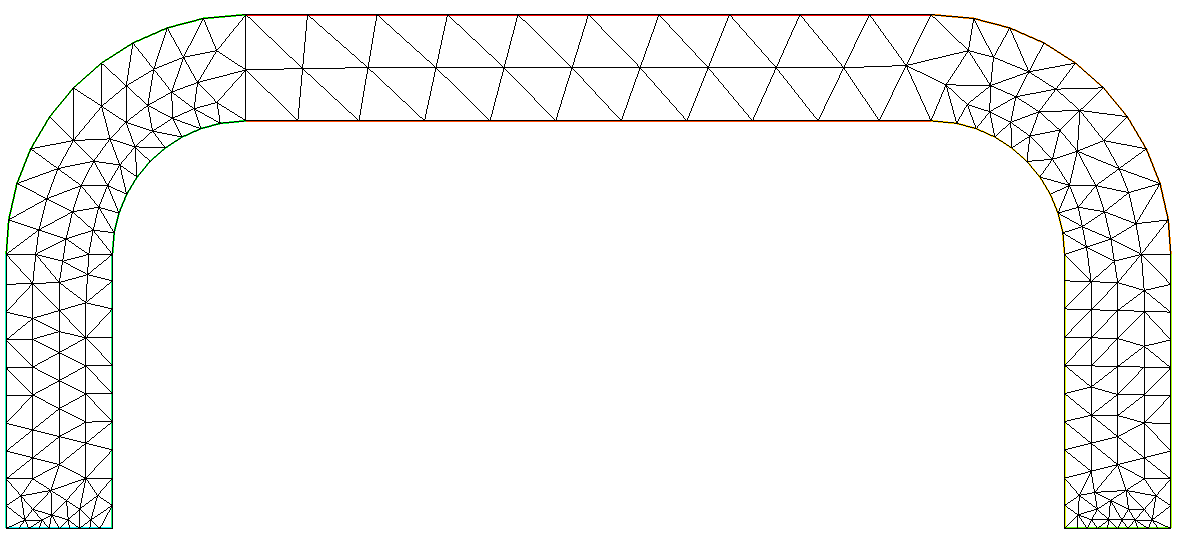
\includegraphics[width=12cm]{imgs/all_maillage_default.PNG}
            \caption{Maillage basique du pont}
            \label{fig:maillage_default}
        
        \end{center}
    \end{figure}

    On remarque cependant sur la figure \ref{fig:maillage_default} que la zone d'intérêt a un maillage très grossier, tandis que les pieds du pont sont très maillés. 
    On choisit donc de pondérer les subdivisions du maillage ($n/2$, $n$ et $2n$), ce qui donne la figure \ref{fig:maillage_pondere}.
    
    \begin{figure}     
        \begin{center}
        
            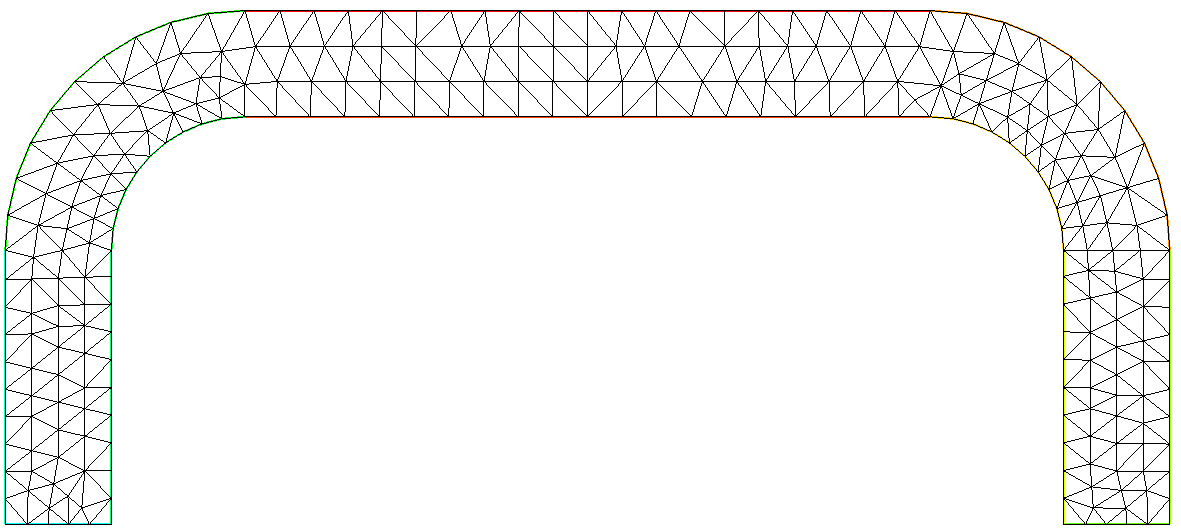
\includegraphics[width=12cm]{imgs/all_maillage_pondere.PNG}
            \caption{Maillage plutôt homogène du pont}
            \label{fig:maillage_pondere}
        
        \end{center}
    \end{figure}

    Ensuite, on donne de la profondeur afin de passer à un maillage 3D avec la fonction \emph{buildlayers} de FreeFem++, 
    avec un paramètre $m=n/2$ qui est le nombre de subdivisions de la bordure du maillage. On effectue après une rotation de la structure 
    avec la fonction \emph{movemesh3}, en pensant à spécifier \emph{orientation=-1} pour ne pas avoir un maillage non conforme.

    On obtient ainsi la figure \ref{fig:maillage_3d}.

    
    \begin{figure}        
        \begin{center}
        
            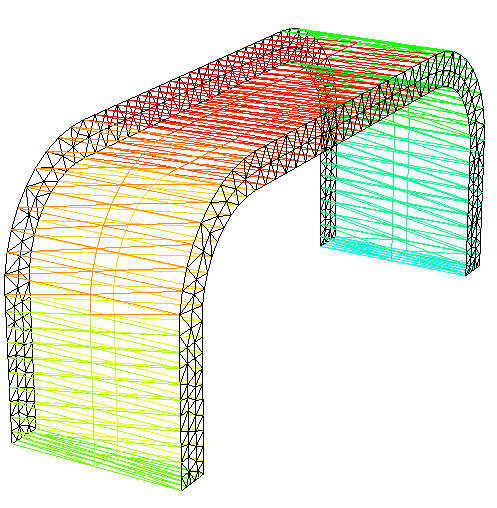
\includegraphics[width=6cm]{imgs/all_maillage_3d.PNG}
            \caption{Maillage 3D du pont}
            \label{fig:maillage_3d}
        
        \end{center}
    \end{figure}

    Après écriture de l'équation \ref{varia} dans le langage de FreeFem++, on obtient le déplacement en P en cherchant la déformation verticale minimum, ainsi que 
    l'aperçu de la structure déformée (Figure \ref{fig:simu_def}).

    On a choisi des éléments $\mathbb{P}_1$ car ce sont les éléments finis les plus simples qui permettent d'obtenir des solutions viables.
    En effet, les éléments finis $\mathbb{P}_0$ (constants) posent problème car il y a la divergence de $\vec{u}$ (dérivées de première ordre).
    Les éléments finis $\mathbb{P}_k, k \geq 2$ sont inutilement compliqués (degrés de liberté) et alourdissent les calculs.

    Sur les figures, $coef$ désigne le coefficient d'amplification du déplacement pour pouvoir l'observer, $dep$ le déplacement en P et $lateral$ 
    le déplacement maximal selon l'axe $y$ (tout est en mètres).
    
    \begin{figure}        
        \begin{center}
        
            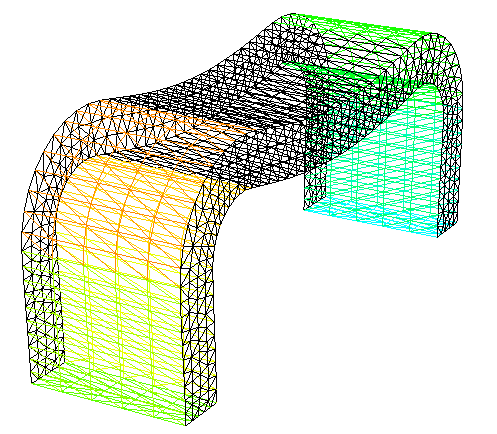
\includegraphics[width=6cm]{imgs/all_simu.PNG}
            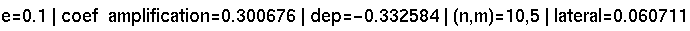
\includegraphics[width=12cm]{imgs/all_simu_label.PNG}
            \caption{Résultat d'une simulation de toute la structure}
            \label{fig:simu_def}
        
        \end{center}
    \end{figure}

    On peut réaliser la même démarche pour la moitié de la structure en utilisant l'équation \ref{moitie} (Figure \ref{fig:simu_def_moitie}).

    \begin{figure}        
        \begin{center}
        
            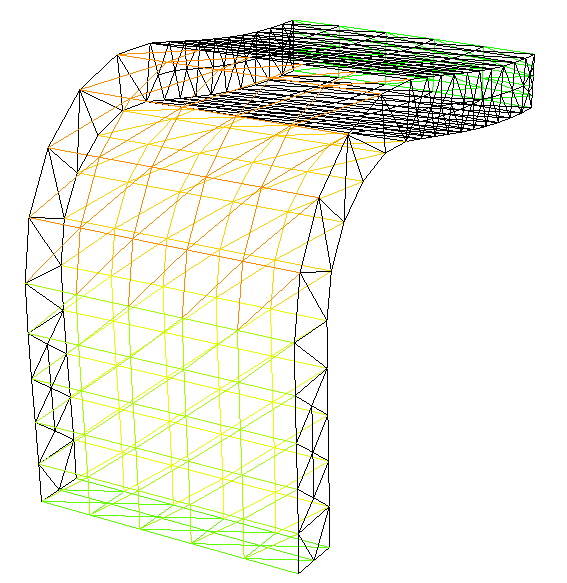
\includegraphics[width=6cm]{imgs/half_simu.PNG}
            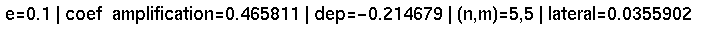
\includegraphics[width=12cm ]{imgs/half_simu_label.PNG}
            \caption{Résultat d'une simulation de la moitié de la structure}
            \label{fig:simu_def_moitie}
        
        \end{center}
    \end{figure}


\begin{problem}{4}
    Retravaillons le maillage pour avoir de meilleurs résultats et vérifier les propriétés de convergence.
\end{problem}

    Nous pouvons remarquer que le déplacement n'est pas le même entre la moitié de la structure et sa totalité (33 cm par rapport 21 cm).
    Cela pourrait donc signaler que le maillage n'est pas suffisamment fin pour que la solution approchée est convergée vers la solution exacte.

    Nous allons donc utiliser trois techniques pour faire converger les fonctions trouvées :
    \begin{itemize}
        \item Un raffinement manuel du maillage. On augmente donc $n$ et $m$ respectivement de 5 et de 2 à chaque itération, en partant de 10 et de 5.
        \item Un raffinement automatique du maillage dans le plan de coupe avec \emph{adaptmesh} et manuel en profondeur. On utilise \emph{adaptmesh} afin d'adapter le maillage 2D
        dans le plan $(xz)$,
                et on augmente $m$ de 2 à chaque itération, en partant de 4. On spécifie 
                notamment une erreur (d'interpolation $\mathbb{P}_1$) sur \emph{adaptmesh} de 0.001 au lieu de 0.01 par défaut afin d'avoir des 
                résultats de convergence plus en accord avec la première méthode, malgré un temps de calcul plus long.
        \item Un raffinement entièrement automatique avec la fonction \emph{mshmet} (retourne une métrique qui va permettre
        d'améliorer le maillage et qui sera passée en paramètre de la fonction ci-après) et \emph{mmg3d}.
            On spécifie là une erreur de 0.0001 au lieu de 0.01, par un choix empirique.
    \end{itemize}
    
    \begin{figure}        
        \begin{center}
        
            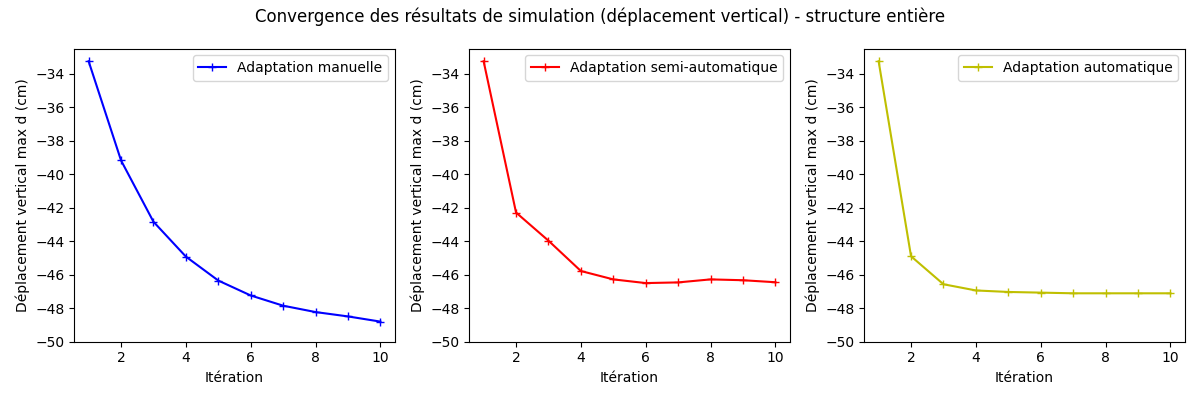
\includegraphics[width=16.5cm]{imgs/cvg.png}
            \caption{Résultats des simulations (structure entière)}
            \label{fig:cvg}
        
        \end{center}
    \end{figure}

    D'après la figure \ref{fig:cvg}, on en déduit que le déplacement réel doit être proche de 48 cm. On constate une petite différence d'asymptote avec l'adaptation manuelle,
    qui pourrait être dûe par exemple par à la lenteur de la convergence ou, de manière plus probable, à des paramètres dans les fonctions d'adaptations du maillage
    (semi-)automatiques pas suffisamment optimisés. Par exemple, diminuer le paramètre erreur $err$ de 0.001 à 0.0001 pourrait améliorer ces méthodes (mais cela aurait un
    coût temporel conséquent). On constate cependant que la vitesse de convergence avec les fonctions d'adaptation de FreeFem++
    et MMG est beaucoup plus rapide (moins d'itérations) avec les paramètres choisis.

    On effectue la même étude de convergence pour la demi-structure (figure \ref{fig:h_cvg}).

    \begin{figure}        
        \begin{center}
        
            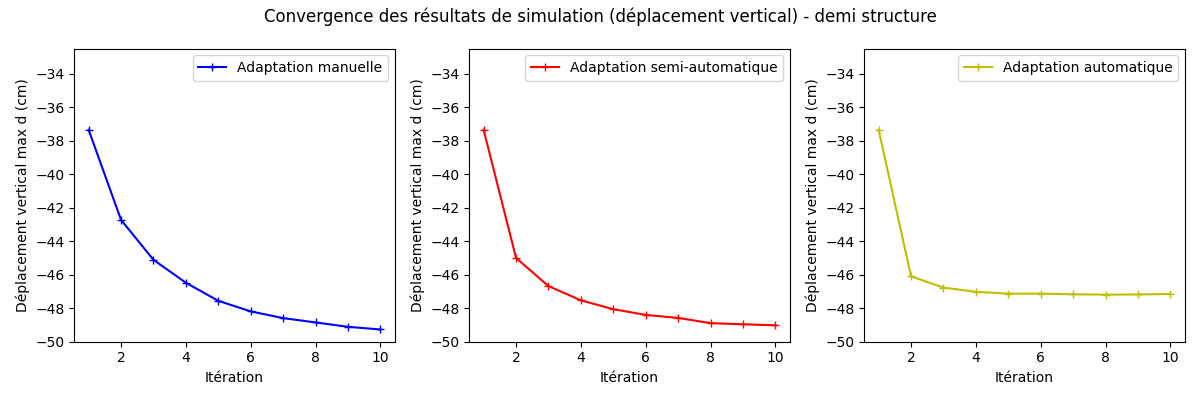
\includegraphics[width=16.5cm]{imgs/cvgH.png}
            \caption{Résultats des simulations (demi-structure)}
            \label{fig:h_cvg}
        
        \end{center}
    \end{figure}

    Les simulations sur la demi-structure sont en accord avec la structure entière (autour de 48 cm).

    Pour la suite des simulations, on choisit donc un maillage manuel avec $n=30$ et $m=15$, qui allie bonnes performances (1 seconde de calcul environ) avec une précision qui semble satisfaisante.
    
    Le détail des techniques d'adaptation de maillage peut être trouvées dans le code, disponible en annexe \ref{source_code}.
    La figure \ref{fig:maillage_auto} montre une adaptation de maillage automatique.
    
    \begin{figure}        
        \begin{center}
        
            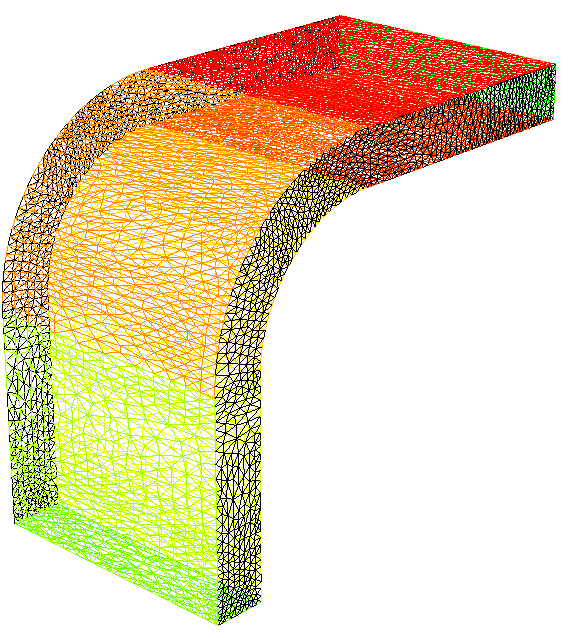
\includegraphics[width=7cm]{imgs/half_maillage_auto.PNG}
            \caption{Exemple de maillage adapté automatiquement (demi-structure)}
            \label{fig:maillage_auto}
        
        \end{center}
    \end{figure}

    Les simulations ont pris quelques minutes pour être calculées. 

    Il aurait pu être intéressant d'utiliser \emph{FreeFem++-mpi} et \emph{MUMPS-mpi} afin d'accélérer les calculs sur nos PCs.
    Il serait également possible de comparer les temps de chaque méthode pour savoir laquelle employée afin d'avoir les meilleures performances avec la meilleure précision.
    Dans tous les cas, il faut spécifier à toutes ces fonctions les "bons" arguments pour obtenir des résultats satisfaisants.

%critique : pas d'adapatation de m

%adapt mesh très mauvais maillage

% parallelization freefem

%optimisation temps

% étude convergence

% problème 2d équivalent
% adaptation de maillage 3d mmg3d et mshmet
% mumps, parallèle autre exécutable freefem
% erreur de valeurd

% bibliographie freefem ?
    \section{Optimisation de l'épaisseur}

    \subsection{Approximation graphique}
    
    Pour commencer à optimiser l'épaisseur du pont, nous avons utilisée l'équation \ref{varia} pour calculer le déplacement en fonction de l'épaisseur. Celle-ci a varié de $0,1$ jusqu'à $0,3$ mètres, sachant que nous avons été limité par le rayon $r = 0,35 m$, avec des incréments de $0,006 m$.
    
    Le graph obtenu est montré dans la \ref{fig:graph} :
    \begin{figure}[H]        
    \begin{center}
	
        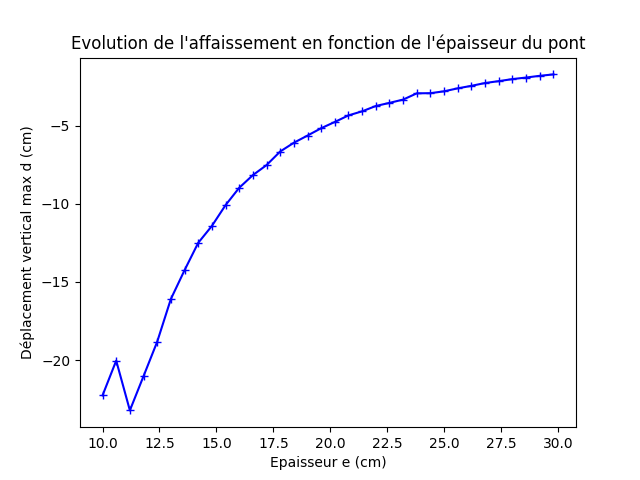
\includegraphics[width=12cm]{imgs/graph.png}
        \caption{Evolution de l'affaissement en fonction de l'épaisseur du pont. Chaque épaisseur utilisée pour le calcul est montré par une croix sur la courbe.}
        \label{fig:graph}
    
	\end{center}
    \end{figure}
    Ce graph montre que à partir de environ $0,15 m$ le déplacement commence a être dans les conditions souhaités. Ce fait nous aide à définir des conditions pour le raffinement des solutions dans la prochaine section, car nous avons un intervalle plus petit à regarder, $[15; 17,5]$ ce qui facilite les calculs.
    \subsection{Raffinement de la solution}
    
    Afin d'utiliser la méthode dichotomie, nous avons défini des variables $e^n_{min}$ et $e^n_{max}$  qui seront utilisé pour calculer une épaisseur moyenne $e^n$ 	qui donnera le déplacement $d^n$. Si:
    
    \begin{itemize}
    \item $|d^n| <= |d_0|$, la valeur moyenne $e^n$ sera la nouvelle valeur de $e^n_{max}$ et $e^n_{min}$ reste constante.
    \item $|d^n| >= |d_0|$, la valeur moyenne $e^n$ sera la nouvelle valeur de $e^n_{min}$ et $e^n_{max}$ reste constante.
    \end{itemize}
   
   À partir du graph montré dans la \ref{fig:graph} généré dans la section précédente, nous avons choisit des valeurs initiales pour $e^n_{min}$ et $e^n_{max}$ de $0,125 m$ et $0,175 m$ respectivement. La valeur de $e^n_{min} était choisi dehors de l'intervalle d'intérêt pour pallier des imprécisions de lecture graphique.
   
   Les calculs ont été fait dans une boucle \emph{while} et la condition de arrêt était : tant que la valeur absolute de $d^n$ est différent de $0.1 m$ \emph{et} la valeur absolute de $|d^n|-0.1$ est plus petite ou égal à $0.001$, les calculs seront faites. Nous avons choisit cette valeur de $0.00001$ par des essais pour avoir un compromis entre une bonne valeur d'épaisseur et le temps de calcul.
    
    Nous avons aussi remarqué que une condition en plus serait nécessaire pour assurer un déplacement plus petit que $ 0.1 m$. De cette façon, l'épaisseur finale sera $e^n_{max}$ et le déplacément sera calculé par rapport à elle. Alors, les valeurs obtenues sont:

    \begin{center}
    $d^n = - 0,0999397 m$
    
    $e^n_{max} = 0,1531125 m$
    \end{center}
    
    \clearpage
    \appendix
    \section {Code source}

    Le code source du programme écrit est disponible sur \url{https://github.com/florian6973/finite-elements-project}.

    On y trouve aussi l'ensemble des ressources utilisées pour la rédaction du rapport.

    %\lstinputlisting[language=FreeFem]{simulation-v2.edp}


    %code + lien github
    
\end{document}
